\documentclass[a4paper 12pts]{article}
\usepackage[utf8]{inputenc}
\usepackage[T1]{fontenc}
\usepackage[francais]{babel}
\usepackage{graphicx}



%macro


\title{Manuel Utilisateur iRover}

\author{R. Joachim CLAYTON}

\begin{document}

\maketitle


\begin{figure}[h]
   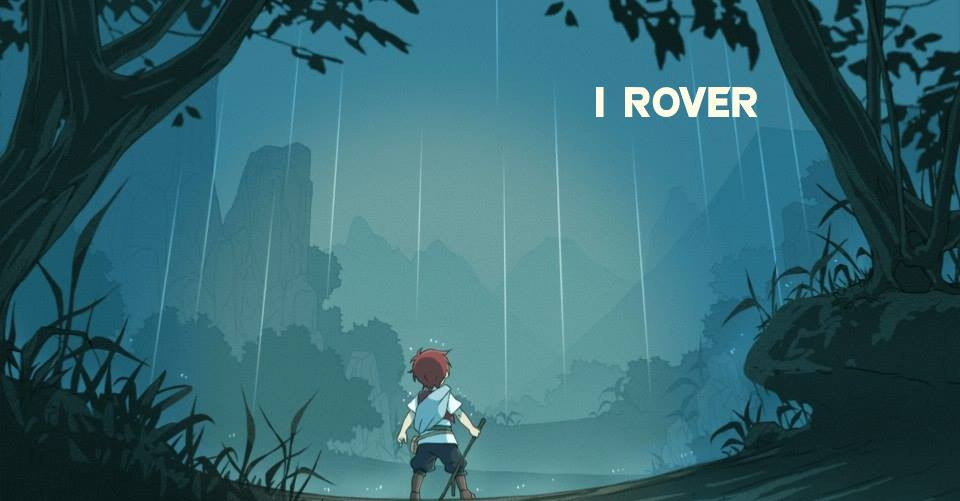
\includegraphics[width=350pt]{Illustration/proj_irover.jpg}
	\caption{iRover, l'histoire d'un héros qu'on appellait robot}
\end{figure}



\newpage


\renewcommand{\contentsname}{Sommaire} 
\tableofcontents

\newpage



\section{iRover, l'histoire d'un héros}

%background, histoire, scénario

\vspace{1cm}

Cette partie est dédiée à l'histoire de notre héros, son monde et ses motivations.
Si vous désirez en apprendre plus, laisser moi vous compter son histoire.

\vspace{1cm}

\subsection{Le monde de Lorr}

\vspace{1cm}

\begin{figure}[h]
	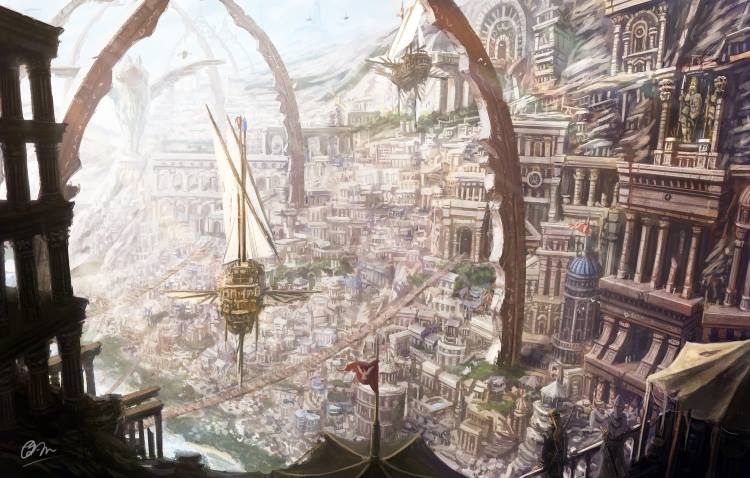
\includegraphics[width=350pt, height=180pt]{Illustration/Lina.jpg}
	\caption{Lina}
\end{figure}

\vspace{1cm}

Le pays de Lorr, vaste étendu de terre fertile entouré de montages et de forêts luxuriantes, abrite la vallée perdu du Vertou, 
là où nul n'a mit les pieds depuis plusieurs siècle.\\
On raconte que c'est ici que le grand pirate du nom de Stevy J. y aurait caché un trésors :"le chamalo magique".\\
Notre héros, intrépide aventurier du nom de Rover quitte alors sa ville natale Lina, où l'industrie et la maitrise de l'acier règne,  et part à la recherche de cette sucrerie antique.\\

\newpage

Cependant  cette mystérieuse vallée est habitée par d'étranges créatures : "des chou-kêtes".\\
Une horde de monstre farouchement attaché à leur territoire connu pour attaquer quiconque y pénetrera.\\

\vspace{1cm}

\begin{figure}[h]
	\includegraphics[width=350pt]{Illustration/vertou.jpg}
	\caption{Vertou}
\end{figure}



\vspace{1cm}


\newpage
\subsection{Stevy J.}

\vspace{1cm}

\begin{figure}[h]
  	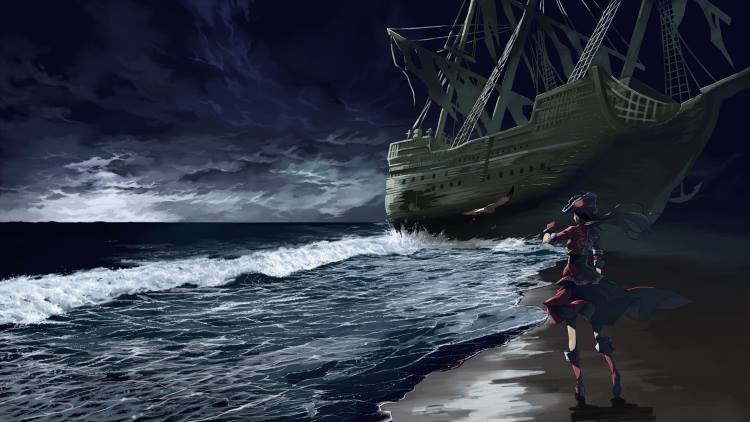
\includegraphics[width=350pt]{Illustration/Steve.jpg}
	\caption{Illustration du bateau de Steve}
\end{figure}

\vspace{1cm}

A une époque lointaine, Steve J Obse de son nom complet, grand pirate et chasseur de trésor, écuma les 8 océans du monde pour venir finir ses jours dans le pays de Lorr.\\
On raconte qu'il aurait réussi à trouver le chamalo magique un artefact qui apporterait gloire, richesse et sucrerie infinie à quiconque le possèdera.\\
Stevy sera capturé et pendu pour piraterie et ne révèlera jamais ses secrets même dans sa biographie post mortem.\\
Beaucoup d'aventurié ont tenté de retrouver son trésor partout dans le monde mais il n'existe qu'un seul endroit où personne n'a mit les pied après le passage du celèbre pirate.



\newpage

\subsection{Rover, un héros pas comme les autres}

\vspace{1cm}

\begin{figure}[h]
  	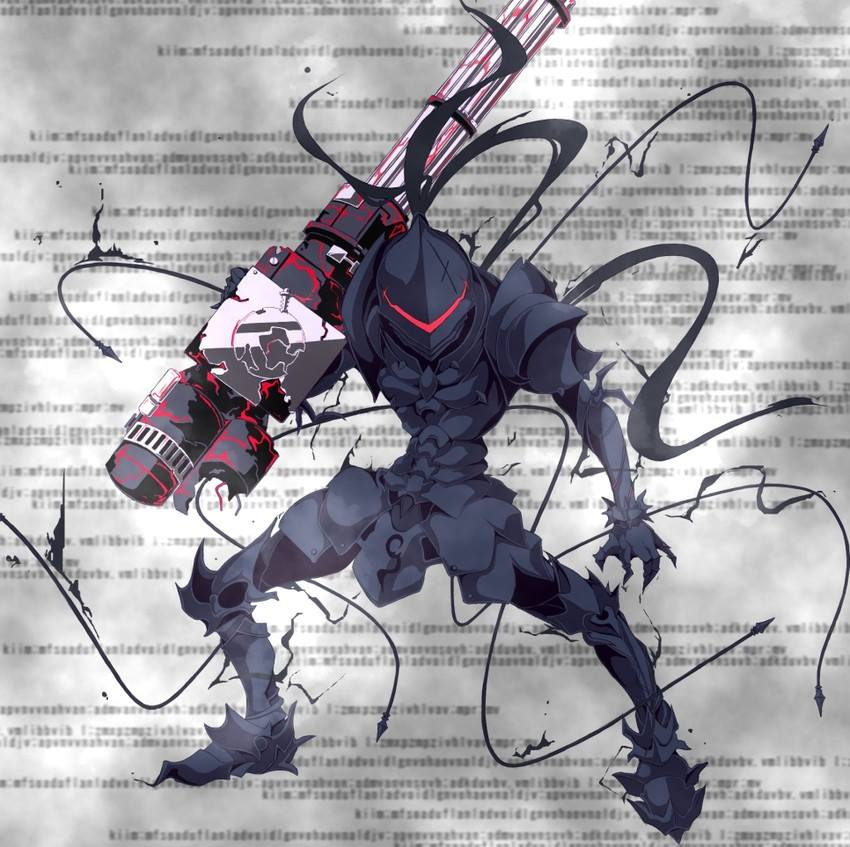
\includegraphics[width=350pt]{Illustration/Rover.jpg}
	\caption{Rover en Armure}
\end{figure}


Rover, notre héros, un apprenti forgerons reve d'aventure ! Ses années d'apprentissage lui permit de créer une armure lui donnant une apparance de robot et surtout augmentant sa protection contre les dangers de la vie au quotidient.
Lors de ses excursions il ne sort jamais sans son arme :  un petit bazooka, une arme de poing d'une très grande puissance.


\subsection{Les Chou-kêtes}
\vspace{1cm}


\begin{figure}[h]
  	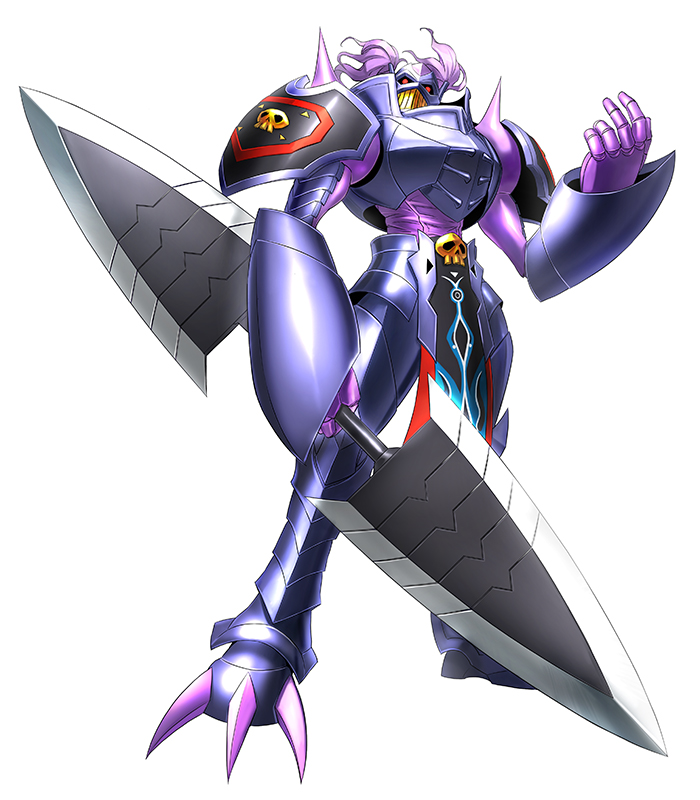
\includegraphics[width=300pt]{Illustration/Badboy.jpg}
	\caption{Général des Chou-Kêtes}
\end{figure}

\vspace{0.8 cm}

Bien des sciècles après la mort de Stevy J. On raconte que des créatures marines surgirent des océans pour venir habité dans la valée.
Personne ne sait exactement qui ils sont, d'ou ils viennent. Le dialogue avec ces êtres est impossible et il ne réponde que par la violence aux étrangers qui
pénetre sur leur territoire.



%regle du jeu

\section{But du jeu}


\vspace{2cm}

L'objectif principal du jeu (ou plutot de notre jeune amis) est de ramasser tous les trésors présents 
sur le terrain afin d'atteindre gloire et richesse et surtout un jour trouver le chamalo magique.\\

Des coffres seront disséminés sur la carte, souvent derrière des obstacles que le héros devra contourner.\\ 
Des ennemis (les chou-kêtes) pourront également attaquer notre héros et donc un combat sans merci s'enclanchera entre héros et monstre.\\


\begin{figure}[h]
   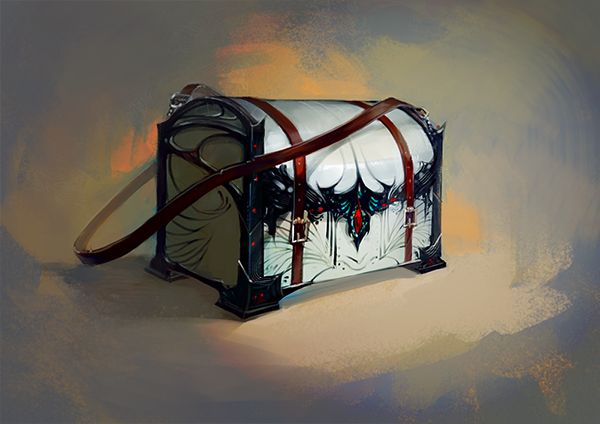
\includegraphics[width=350pt]{Illustration/coffre.jpg}
\caption{coffre au trésor}
\end{figure}


Le jeu prendra fin une fois tous les coffres ramassés ou si notre héros ne peut plus continuer son aventure.




\newpage

\section{Manuel d'installation}

\vspace{1.5cm}


\subsection{makefile}

%expliquer l'installation

%expliquer les librairies à utiliser
%parler de l'option pour que ça compile avec tout les systemes d'exploitation

\subsubsection{gestion des systeme d'exploitation}

\subsection{.config ????????}
%a virer si on utilise pas
%les options du makefile
%a ambélir si on a des idées (rappelle que meme si c'est pas implémenté, ça peut nous donner des points)


\newpage

\section{Documentation utilisateur}

%documentation utilisateur : donner des informations à des utilisateurs lambda sans grande connaissance informatique, avec des mots simple sur le fonctionnement de l'application.
%donner egalement une description simple de comment est faite ou est géré les partie de l'application.


Cette partie est dédiée aux utilisateurs recherchant à comprendre les méchanismes de cette petite application.
Si vous voulez des détails technique merci de vous referrez au Manuel Technique.
Nous vous expliquerons ici comment les divers élément du jeux s'articule afin de vous permettre une meilleur expérience utilisateur.


\subsection{Les personnages}
Le jeu possède deux type de personnages: 

\begin{enumerate}
\item le héros, notre rover ou petit robot
\item les ennemis, les chou-kêtes.
\end{enumerate}

Ces deux type de personnages peuvent à la fois :

\begin{enumerate}
	\item se déplacer, avancer case par case 
	\item combattre, lancer un combat
\end{enumerate}

Chaque personnage possède des coordonnées indiquant leur emplacement en temps réel sur la carte ainsi que des statistiques mais aussi possèdera une armure ainsi qu'une arme.

\subsubsection{Le robot, Rover}


Le robot, en plus de pouvoir se déplacer sur le terrain, peut aussi ramasser des clefs et ouvrir des coffres.
Pour celà, le robot possède un entier nommé "inventaire" qui représente le nombre de clefs que possède le robot à un instant.
Lorsque la fonction ramasser(Clef* clef) est appelée, l'inventaire du robot va s'incrémenter de 1 et lorsque la méthode ouvrir(Coffre* coffre)
est appelée, l'inventaire va se décrémenter de 1.

Rover, notre héros, est controlé par une intelligence artificiel d'où son petit surnom de robot.
Il pourra se déplacer sur la carte, case par case et rencontrera des obstacles. 
N'ayant pas appris à nager et du à des crises de vertiges récurente, il ne pourra ni se déplacer sur l'eau ni grimper sur les rochers,
les arbres, les murs et même les buissons !
Il pourra interagir avec d'autre éléments du monde comme ramasser des objets au sol, se battre contre les ennemis et ouvrir les coffres. 

\subsubsection{les ennemis}

Les ennemis ont les mêmes propriétés que la classe Personnage, c'est juste leur manière de se déplacer qui change par rapport au robot. 
Un ennemi peut se déplacer sur toute la carte de manière aléatoire grâce à un algorithme qui génère un déplacement aléatoire.
Lorsqu'un ennemi est proche du robot, un combat se lance entre les deux personnages.



Certains ennemis seront présent sur le terrain et mettrons le robot en difficulté. 
Le robot devra alors combattre ces ennemis s'il les rencontre afin de rester en vie.
Lorsque le robot se trouve à côté d'un ennemi, il est obligé de le combattre. 
Celà se traduit par un algorithme de combat qui fera gagner le duel au robot ou à l'ennemi. 
Une fois l'ennemi vaincu, celui-ci disparait du terrain mais dans le cas contraire, 
notre héros ne sera plus en mesure de continuer et notre jeu prendra fin.

\subsection{les coffres}

\subsection{les clé}

\subsection{L'environnement}
La carte sur laquelle le robot se déplace est construite à l'aide de Tiled, il s'agit d'un logicielle permettant de créer des cartes case par case. 
Pour les cartes modélisées, on distingue deux types de cases:

L'environnement comprend la gestion des coffres et des clefs.
Une clef possède des attributs positionX et positionY qui sont ses positions en X et en Y sur la carte. 
Un coffre possède les mêmes attributs mais un statut en plus qui est simplement une valeur booléenne qui dit si le coffre est ouvert ou fermé.


\begin{enumerate}
	\item les cases ou le robot peut se déplacer
	\item les cases ou le robot ne peut pas se déplacer
\end{enumerate}

La carte est sous forme d'un fichier XML que le programme interprête pour renvoyer une carte exploitable par le robot.

L'environement servira de base également pour la disposition des autres entités présente, coffre, clef ennemie.
Ceux ci sont disposé aléatoirement sur la carte à des endroits accessibles par le héros mais ils ne peuvent pas se déplacer.
La rencontre avec un de ces éléments entraine la gestion des évênements.





\subsection{La gestion des évênements}

Le robot, notre amis rover, devra faire face à beaucoup d'évênements, ouvrir un coffre, se battre contre un ennemi, ramasser une clef, se cogner contre un mur etc..
Tout ceci est géré par le comportement de chaque objets mais aussi pour sa hierarchi sur la carte.

\subsubsection {Rencontre avec un ennemi} 
Un ennemis et notre héros devront avoir la même importance physique : il ne peuvent pas se supperposer.
Un ennemis et notre héros n'auront besoin que d'un regard pour enclanché le combat ! 1 case de différence.

%mettre un schéma

\subsubsection {Ouvertude d'un coffre}
Un coffre et notre héros n'ont pas la même importance physique : le héros devra pouvoir "marcher" sur le coffre.
Un coffre et notre héros devront impérativement être sur la même case pour que le coffre puisse s'ouvrir et ce dernier, 
le héros, devra avoir une clé pour que cela soit possible.

%mettre un schéma

\subsubsection {Ramasser une clé}
Une clé et notre héros n'ont pas la même importance physique : le héros devra pouvoir "marcher" sur la clé.

%mettre un schéma
 
\subsection{l'interface utilisateur}

\subsection{IA}

\subsubsection{path finding}

\subsubsection{découvert de la carte}

\subsection{condition fin de jeu}





\section{tutoriel}

\end{document}


